\chapter{Literature Review}\label{Literature Review}

\section{The Media}

\subsection{Role of the Media in a crisis}\label{Role of the Media in a crisis}

It is not an easy task to quantify how much the media impacts a society's perception on various topics, events and personalities especially given the large span of time it has been around for. However what is clear is that major events are dealt or handled with a goal to have it reported in certain ways by news outlets. When considering that world leaders constantly think about how certain decisions will be reported by news outlets, amongst other examples and situations, it is fair to state that the news media clearly affects how society works to this day. 

"Cultivation theory" is a term which was introduced by \cite{gerbner1976living}. It represents the idea that regular exposure to media, in the context of their study, television media, influences the viewers idea and perception of everyday life events. Through the analysis of answers from both light and heavy consumers of media they were able to quantify the difference in perspectives as seen in Figure \ref{fig:tv perception} which shows one of their experiments. While this figure illustrates the immediate difference in perceptions that heavy media consumption can cause, it also has been found to have long-term effect on an individuals behaviour. These changes are found to be slow and mostly indirect but sum up to significant changes in an entire population over a long period of time.

\begin{figure}[H]
      \centering
      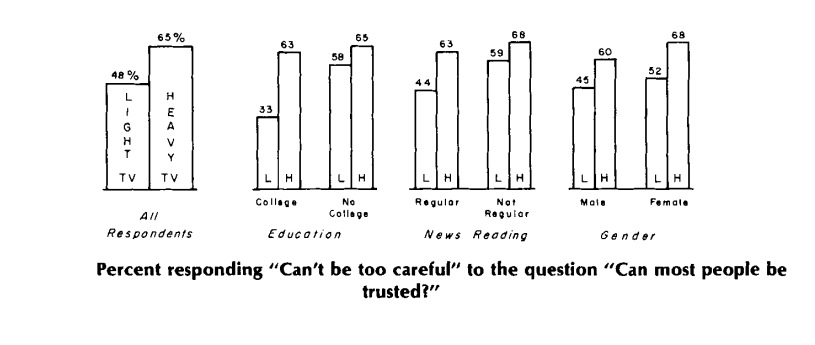
\includegraphics[scale=0.65]{lit_review/tv_2.png}
      \caption{Perception Difference of Light and Heavy TV Consumers}
      \label{fig:tv perception}
      \emph{Source: \cite{gerbner1976living}}
\end{figure}

In the context of a crisis of global scale such as the COVID-19 pandemic, the news media play a particularly important role as they diffuse information which may be critical to its readers survival. Studies have analysed how news agencies handled this situation and found conflicting news being published particularly at the start of the pandemic. Finding "large differences in content between the two most popular cable news shows in the US" \citep{bursztyn2020misinformation}, the study also found that areas where news agencies downplayed the impact of COVID-19 resulted in more cases and deaths. A different study analysed sentiment polarity for COVID-19 news coverage over Europe and found France to have a large number of positive news in comparison to Eastern European countries (Figure \ref{fig:eu mood}). This same study found France to have the highest rate of headlines being classified as negative through the use of a pre-trained multilingual BERT\footnote{\url{https://github.com/google-research/bert}} model. Finding a rate of 50\% of headlines being classified as negative \citep{robertson2021covid}.
Finally, an analysis on US  news discovered differences in news polarity and politicization of news depending on the format, stating that "newspaper coverage is highly politicized, network news coverage somewhat less so, and both newspaper and network news coverage are highly polarized [...] politicians appear in newspaper coverage more frequently than scientists, whereas politicians and scientists are more equally featured in network news" \citep{hart2020covid19}. The political situation is very different in France than the US however the polarity of news seems to be common as we've just seen that 50\% of French news headlines were labeled as negative by \cite{robertson2021covid}.

\begin{figure}[H]
      \centering
      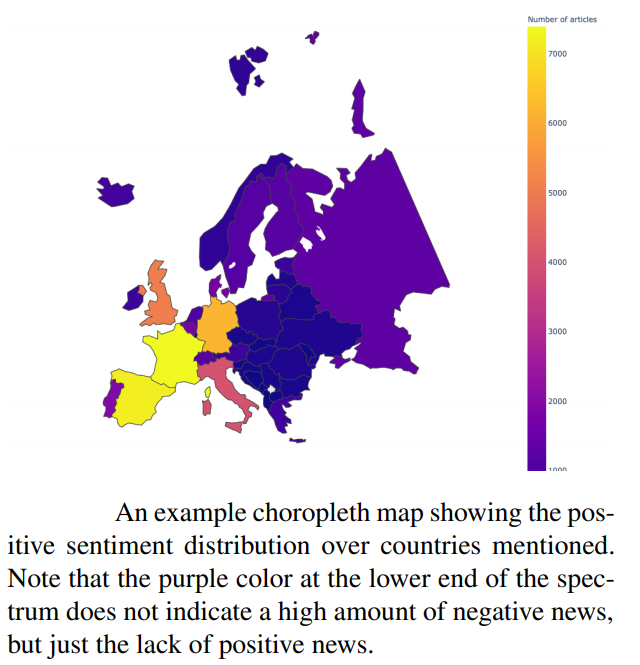
\includegraphics[scale=0.65]{lit_review/eu_2.png}
      \caption{Positive Sentiment Distribution of COVID-19 News in Europe}
      \label{fig:eu mood}
      \emph{Source: \cite{robertson2021covid}}
\end{figure}

\subsection{French News History}\label{chap:French Press}

France played a major role historically with regards to how news works today. Its first newspaper \emph{Gazette} was founded in 1615 under to reign of king \emph{Louis XIII}. Later in 1835 the \emph{Agence Havas}, now known as \emph{Agence France Presse} was founded. It is the world's oldest news agency and is still active on an international scale to this day. It was founded some years before the law of 29 July 1881 on the freedom of the press which provided a framework for news agencies to publish articles, although amends have been made, this law is still active to this day. Today, news agencies play a major role in news distribution worldwide, they gather news and create reports that are then sold to news organisations such as newspapers, TV companies, governments and more. To this day, four companies own most of the world's information, Agence France Presse (AFP), Associated Press (AP), Reuters and United Press International (UPI).

Through the various regimes, dictators and republics since 1615, the importance of the press went through ups and downs. Some periods included high censorship such as under the French Directory (during the first republic), followed by \emph{Napoléon Bonaparte} (also known as \emph{Napoléon Ier}) who closed most news agencies and used the remaining for spreading propaganda. It also went through brighter periods such as under the third republic of 1871-1929 where it was easier and cheaper to mass produce newspapers and news outlets were uncensored. The last event to have happened historically to French news was during World War 2. During the occupation of German troops, the French Government moved to the city of Vichy (also known as the \emph{Government of Vichy}), collaborationist newspapers have emerged, all of which were taken control of once France was liberated.

\section{Sentiment Analysis}\label{Sentiment Analysis}

Sentiment Analysis (or opinion mining), is "the task of finding the opinions of authors about specific entities" \citep{feldman2013techniques}. It is a sub-field of Natural Language Processing (NLP) which has been growing in interest on a worldwide scale for over 15 years thanks to its vast range of use cases (Figure \ref{fig:sentiment interest}).

\begin{figure}[h!]
      \centering
      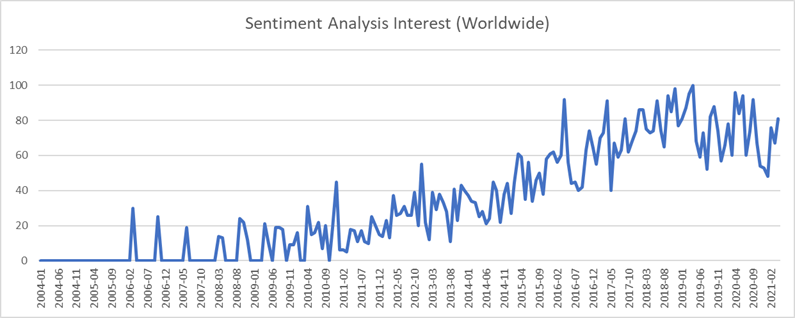
\includegraphics[scale=0.65]{lit_review/sentiment_analysis_interest.png}
      \caption{Sentiment Analysis Interest}
      \label{fig:sentiment interest}
      \emph{Source: Google Trends}
\end{figure}

In fact, sentiment analysis has been used in a wide range of topics, including political analyses of social and news media \citep{ahmad2011new}, stock market behaviors \citep{rao2012analyzing,li2014news}, customer sentiment \citep{cambria2013new,mouthami2013sentiment}, fake news detection \citep{bhutani2019fake} and countless more applications.

Languages are full of ambiguity and in particular the French language as some words can have drastically different meanings even though they are written the same, or adding an accent from a large variety of options can drastically change the meaning of a word. On top of this, a select set of words make up the majority of text, in fact, using a frequency-rank, it was found that the first 100 words make up for about 50\% of all of the words in a text cluster \citep{ahmad2007being}, while this number may vary for the french language, this observation means that the interpretation of these highly frequent words is key to extracting sentiment proxies from text. Short texts such as tweets \citep{chandrasekaran2020topics} or customer reviews can include a single sentiment or topic. That is not always the case though, as the length of text grows more conflicting opinions are likely to be found. A simple example of this can be found in a customer review for a product: "I liked using the product, however I wish it didn't break after a day" where clearly both a positive and negative sentiment can be extracted from this review. This shows that there are multiple ways to perform sentiment analysis on text. A document-level approach computes the overall sentiment of a piece of text such as a tweet or a review, on the other hand, a sentence-level analysis approach can also be taken where a distinction is made between factual sentences (objective phrases) and subjective sentences which mostly contain opinions (subjective phrases) \citep{wilson2009recognizing}. A sentence-level approach is often used for tasks such as text summarizing, on the other hand, a document-level approach is often used for reviews or social media posts. 

Thankfully, some NLP techniques have now been standardised to help with these issues. One of the most important ones being the use of stemming or lemmatising.

\subsection{Stemming and Lemmatising}
\label{lemmatization}\label{stemming}

Both of these techniques at their core attempt to obtain the same result: to simplify a word into a more basic form, the difference lies in how that is performed. Stemming trims a word into its word stem, on the other hand, lemmatising is more complex and transforms a word into its its dictionary form. Table \ref{tab:stem and lemma} shows an example of both techniques. The most popular stemming approach is the five-step Porter Stemmer \citep{porter1980algorithm}. This algorithm however does not apply to languages other than English. With regards to lemmatising, rule-based taggers are very commonly found, these probabilistic models have obtained high accuracy and are very commonly used \citep{brill1992simple}. This project makes use of TreeTagger, a multilingual tagger implemented using decision trees \citep{schmid2013probabilistic}. Another tool, SpaCy\footnote{\url{https://spacy.io/}}, an open source multilingual package which includes a lemmatizer was also used. After some comparison, it was found that the SpaCy implementation resulted in a higher rate of word matching so it was ultimately used to compute the results throughout this study.

While stemming is much easier to apply, much more efficient to compute and does not require context, it can miss valuable information, especially when applied to the French language which contains a very high amount of irregular verbs or adjectives. This can be seen in the example shown in the table comparing both approaches (Table \ref{tab:stem and lemma}). On the other hand, lemmatising is much harder to apply as it requires context of the word in question within the sentence. However it is also much more representative of the meaning of each word. 

\begin{table}[H]
\centering
\begin{tabular}{@{}ccc@{}}
\toprule
\textbf{Input} & \textbf{Stem} & \textbf{Lemma} \\ \midrule
Livre (to deliver) & livr & livrer \\
Livre (a book) & livr & livre \\ \bottomrule
\end{tabular}
\caption{Comparison of Stemming an Lemmatising}
\label{tab:stem and lemma}
\end{table}

\subsection{Computing Sentiment}

There are two main approaches to performing sentiment analysis, Lexicon based and Machine Learning (ML) based. Both approaches are sometimes combined to form hybrid methods.

\subsubsection{Machine Learning}

Machine learning approaches require a set of labelled training data in order to train a model. Often the quality and size of the training data is key to obtaining results of high accuracy, however these approaches often work on a specific data set and it is much harder to generalise to types of texts that differ significantly from the original data set. For example the weights associated to a machine learning model classifying customer reviews may be very different from classifying news articles as the vocabulary used can be expected to be quite different. When labelled data is unavailable it is possible to train unsupervised machine learning models, however it was found that "supervised methods undoubtedly perform better than other approaches" \citep{navigli2009word}. This study also points out the fact that relying on large training data sets to train those models in different domains, languages and tasks is not realistic to assume as previously pointed out. In fact this study makes the estimation that "to obtain a high-accuracy wide-coverage disambiguation system, we probably need a corpus of about 3.2 million sense-tagged words" which is unrealistic to create manually. In fact the duration of tagging the words of a corpus manually has been estimated previously, "experience [...] suggests that it takes one person one minute to tag one instance of
a word in a corpus (assuming all instances of the same word are tagged in succession)" \citep{do2000designing}. At the rate of one word per minute this task would take about 27 years to obtain a corpus of the size specified.

Popular machine learning models for sentiment analysis include (but is not limited to) Naive Bayes, Support-Vector-Machine (SVM), Neural Nets, K-Nearest neighbours. Some studies have compared some of the above models in specific classification tasks \citep{wawre2016sentiment,ye2009sentiment,seo2020comparative}.

When using a machine learning approach a decision also needs to be made with regards to the output of a model. Most of the sentiment machine learning models are classifiers, giving an output of true or false. This is partially due to most of the available data sets for sentiment classification being labelled as such. It is in fact much harder and more effort to form a labelled corpus such as to train a regression model as the labelling of each article requires an associated score instead of a boolean value. However, while a classifier may work well for customer reviews or tweets, using regression can be favorable in some tasks such as news articles analysis which are more complex in nature and can rarely be summarised to "positive" or "negative". Hybrid methods have been used in this situation by using the output of lexicons into machine learning models and found it to improve the predictions precision \citep{kolchyna2015twitter}.

\subsubsection{Lexicon}

A lexicon based approach relies on a predefined dictionary where each term is associated with a sentiment polarity and possibly a strength (or weight). The neutrality can be one of "positive", "negative" or "neutral", some dictionaries use a uniform weight distribution which essentially counts the occurrences of a lexicons words and others use a weighting system where a weight is computed for each word based on varying reasons. It is also referred to as the "Bag-of-words" approach as it splits documents into tokens as part of the text vectorization process (the process of converting words into a numeric representation). The polarity of a document is then computed by retrieving the number of word occurrences both in the lexicon and document, where each word is associated with a predefined polarity within the lexicon.

A lexicon approach is usually much easier to apply than a machine learning model and is usually more efficient. Studies have compared both methods, some found lexicon approaches to be more precise or found comparable results \citep{dhaoui2017social,mukhtar2018lexicon}, others found machine learning approaches to be more accurate \citep{kolchyna2015twitter,nasim2017sentiment}.

Studies making use of a lexicon based approach generally make use of dictionaries created by computational linguists which are peer reviewed to ensure quality. A number of popular lexica are available in the English language. This is not always the case for other languages such as French, however, it was found that "online tools can be used to get high quality resources with low cost" \citep{abdaoui2017feel}, this study analysed the performance of online translation tools for translating such dictionaries and found an accuracy of over 90\%. Such general dictionaries work well when analysing a general data set, specialised domains such as science or finance will require the use of specialist dictionaries in addition to the general dictionary as words such as "virus" may be associated with a negative sentiment in a general dictionary but is not considered negative is a scientific context.

An issue with this approach is the handling of negation which is still an issue to this day, where words such as "not" or "so" can be used to negate or put emphasis on a word. Lexicon based sentiment analysis fails to handle such cases correctly \citep{le2014distributed}. Hybrid methods using machine learning have been found to keep such relationship between words \citep{mikolov2013exploiting}. On the other hand, algorithms have been developed for better negation handling in lexicon based approaches \citep{diamantini2016negation}.


\section{French Lexica}\label{French Lexicons}

As previously mentioned, there are few published French general dictionaries, three of which have been used in this study.

\subsection{FEEL}\label{chap: feel}

The French Expanded Emotion Lexicon (FEEL) \citep{abdaoui2017feel}, is a lexicon that is built from the semi-automatic translation of the English NRC Word Emotion Association Lexicon \citep{mohammad2013crowdsourcing}. The study started by querying online translation tools to create a first version, then, "a human professional translator manually validated the automatically obtained entries and the associated emotions" \citep{abdaoui2017feel}. It was found that over 94\% of entries were correct in the first version. This study makes available the obtained dictionary and concludes that it is possible to obtain consistent, quality dictionaries with the use of online translation tools. One of the authors, Amine Abdaoui, was helpful and provided useful pointers on how best to apply the FEEL lexicon in this study through an email conversation.

Word entries of the FEEL lexicon include a polarity of positive or negative as well as a set of emotions: joy, surprise, anger, disgust, sadness and fear. The associated weight for each of these emotions is either 0 or 1. More than 80\% of word entries include a single term, with the remaining mostly consisting of two terms and a minority consisting of three terms.

\subsection{Polarimots}\label{chap: polarimots}

Polarimots \citep{gala2012propagation} is a lexicon that has been constructed semi-automatically, consisting of 7,483 entries. An initial set of manually annotated adjectives were created, from which the propagation of polarity was applied. It was found that "spreading polarities is accurate for 78.89\% of the families with a unique adjective" \citep{gala2012propagation}.

With each word entry is associated its word type (noun, verb, adjective or adverb) as well as a reliability metric of either 33\%, 66\% or 100\%. Finally, 100\% of its entries are composed of single words.

\subsection{Diko}\label{chap: diko}

Diko is a lexicon that was built form a game: "LikeIt". LikeIt is "a GWAP (Game With A Purpose) that allows to attribute a positive, negative or neutral value to a term, and thus obtain a resulting polarity" \citep{lafourcade2015collecting}. Because of the nature of the lexicon, Diko is very large. With each word entry, is associated the number of positive, negative and neutral votes. Diko differs significantly from other lexicons as terms are not lemmatized and only 33\% of its terms are single words, with some terms including more than 6 individual words \citep{abdaoui2017feel}. Diko is also the largest and has been found to include 97\% of FEEL terms and 98\% of Polarimots terms.

\section{Statistical Methods}\label{Statistical Methods}

The use of various statistical methods represent a key element for this thesis, as specified in the research objectives (Chapter \ref{chap: Research Objectives}). Such methods provide the link between observed values and identifying potential relationships.

\subsection{Core Statistics}

This first section introduces key, core statistic measures which are used throughout this thesis.

\subsubsection{Mean}

The mean is a very well known statistical measure which consists of the sum of the deviation of all of the values in a sample by the size of that sample. In other words, it is the average value in a sample. It is commonly referred to as $\bar{x}$ for a sample as well as $\mu$ for a population.

\begin{equation}
    \bar{x} = \frac{1}{N}\sum^{N}_{i=1} x_{i}
\end{equation}
Where N is the sample size and $x_{i}$ represents the ith value in the sample.

\subsubsection{Variance and Standard Deviation}

The standard deviation and variance are related. A common symbol for the standard deviation is $\sigma$ for a population and $S$ for a sample. Given the standard deviation $S$ or $\sigma$ then the variance is its squared value: $S^{2}$ or $\sigma^{2}$.

The standard deviation measures how much data diverges from the mean. A low value indicates that the data is clustered around the mean, on the other hand a high standard deviation indicates that the sample is more spread out. The variance also measures how distributed data is relative to the mean in the same manner, except in much larger values as it is squared.

The mathematical formulas for computing the standard deviation and variance for a sample are the following:
\begin{equation}
    S = \sqrt{\frac{\sum_{i=1}^{N}(x_{i} - \bar{x})^{2}}{N - 1}}
\end{equation}
\begin{equation}
    S^2 = \frac{\sum_{i=1}^{N}(x_{i} - \bar{x})^{2}}{N - 1}
\end{equation}

\subsubsection{Skewness}

Similar to the variance and standard deviation, the skewness also measures data distribution. The skewness measures the degree of asymmetry from a normal distribution, in other words, it quantifies the difference between a sample distribution and the normal distribution.

Hence, the skewness for a normal distribution is 0. A positive skewness indicates that the data is skewed to the right, in other words the right tail is longer than the left. On the other hand, a negative skewness indicates that the data is skewed to the left. Figure \ref{skewness fig} illustrates this concept. Mathematically, it is written as such:

\begin{equation}
    skewness = \frac{\sum_{i=1}^{N}(x_{i} - \bar{x})^{3}}{(N - 1) * S^{3}}
\end{equation}
Where N is the sample size, $x_{i}$ is the ith data point from the sample, $\bar{x}$ is the mean and $S$ is the standard deviation.

\begin{figure}[h!]
      \centering
      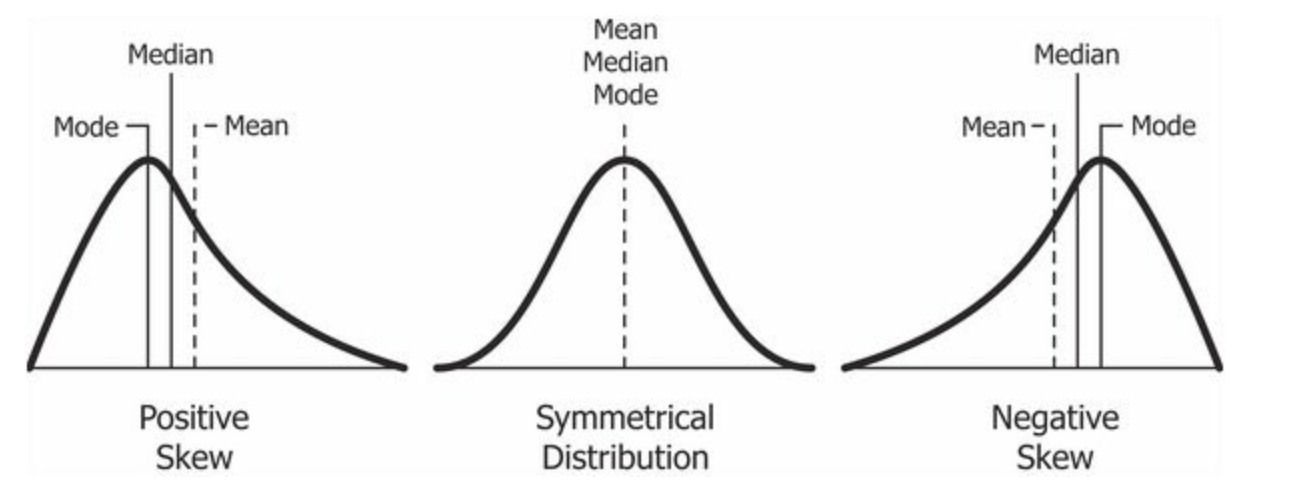
\includegraphics[scale=0.8]{lit_review/skewness.png}
      \caption{Skewness Visualisation}
      \label{skewness fig}
      \emph{Source: Wikipedia}
\end{figure}

\subsubsection{Kurtosis}

Kurtosis is a measure of whether a sample is heavily tailed or lightly tailed relative to a normal distribution. A high kurtosis value infers that a data set will have a large amount of outliers. On the other hand a low kurtosis value indicates a data set with very few outliers. The kurtosis for a standard normal distribution is 3, hence a metric often used is referred to as the "excess kurtosis" and takes the value $kurtosis - 3$.

Mathematically, the kurtosis value is calculated as such:
\begin{equation}
    kurtosis = \frac{1}{N - 1} \frac{\sum_{i=1}^{N}(x_{i} - \bar{x})^{4}}{S^{4}}
\end{equation}

\subsubsection{P-Value}

The P-Value is used in null hypothesis significance testing. Assuming a null hypothesis $H_{0}$, a hypothesis of no difference, and a second hypothesis $H_{1}$, representing the opposite of the null hypothesis. The P-Value is the probability of finding greater results when the null hypothesis $H_{0}$ is true. A level of significance is picked, typically one of 0.1, 0.05 or 0.01. A p-value below the threshold implies that we can conclude that there is significant evidence to reject the null hypothesis $H_{0}$. This study uses a significance level of 5\% (p-value of 0.05) unless specified otherwise.

\subsubsection{Correlation}

This study makes use of the Pearson product-moment correlation coefficient. Correlation (r) quantifies linear relationship between two data sets. Its values range between -1 and 1. A correlation value of zero indicates no linear relationship between the two sets of data. A positive correlation indicates that both variables move in the same direction, it shows that when one becomes larger or smaller, so does the other. On the other hand, a negative correlation shows the opposite: both variables move in the opposite directions. 
A larger distance between zero and the correlation value indicates a stronger relationship, this is true for both positive and negative correlations. The coefficient can be computed using the formula below.

\begin{equation}
    r = \frac{\sum_{i=1}^{N}(x_{i} - \bar{x})(y_{i} - \bar{y})}{\sqrt{\sum_{i=1}^{N}(x_{i} - \bar{x})^{2}\sum_{i=1}^{N}(y_{i} - \bar{y})^{2}}}
\end{equation}
Note that both sets of data must be of the same size. Here N is the sample size of both x and y data sets, $x_{i}$ and $y_{i}$ are the ith data point for data sets x and y respectively, finally $\bar{x}$ and $\bar{y}$ are the means for both data sets.

\subsubsection{Z-Score}

The Z-Score (Z), also known as the standard score, is a value which shows a measure of the a value's relationship to the mean of the data set it belongs to. It represents the number of standard deviations by which a value is above or below the mean value.

\begin{equation}
    Z = \frac{x - \bar{x}}{S}
\end{equation}
Where x is a value of the data set, $\bar{x}$ is the mean and $S$ is the standard deviation.

\subsection{VAR Analysis}\label{chap:var lit rv}

This section introduces the Vector autoregression (VAR) statistical model as well as related statistic measures useful in order to test and evaluate VAR models.

\subsubsection{Vector AutoRegression}

VAR models were originally discovered and used for forecasting economic time series. Since its inception, VAR models have been used in various different applications successfully with some including sentiment analysis proxies \citep{georgoula2015using,zhao2015computational}. VAR works by using previous values of a time series in order to forecast future values.

%Two types of variables:
%Endogenous variables have values that are determined by other variables in the system
%An exogenous variable is a variable that is not affected by other variables in the system.

\subsubsection{Lag Selection}\label{chap:lag selection lr}

There are three popular approaches to selecting a lag order. The Akaike Information Criterion (AIC), which finds the lag being optimal where the associated value is the lowest. The Bayesian Information Criterion (BIC) is the second approach which makes use of Bayes' theorem. It computes the posterior probability of each model such as to find the optimal model. The third criteria is the Hannan-Quinn criterion (HQC) which also has a very similar mathematical formula.

Where L is the maximum value from the likelihood function, k is the number of estimated parameters, the three approaches can be computed as such:

\begin{equation}
    AIC = 2k - 2ln(L)
\end{equation}
\begin{equation}
    BIC = ln(n)k - 2ln(L)
\end{equation}
\begin{equation}
    HQC = 2kln(ln(n)) - 2ln(L)
\end{equation}


In terms of which criterion to trust, the AIC is commonly seen as the most accurate, with the exception of HQC for large sample sizes. There are different advantages linked to each approach in specific situations. Due to this our study shall use the AIC criterion when it is close or equal to HQC on a case by case basis.

\subsubsection{\boldsymbol{R^2} and Adjusted \boldsymbol{R^2}}

Both $R^2$ and the adjusted $R^2$ are statistic measures useful when evaluating a model. They show how accurately a model fits its data. The difference being that adjusted $R^2$ also depends on the number of independent variables in the model. Adding more variables to a model will increase both the $R^2$ and adjusted $R^2$ values if those variables improve the model, on the other had the measures will decrease when the added variables make the model predictions worse.

\begin{equation}
    R^2 = 1 - \frac{RSS}{TSS}
\end{equation}
Where RSS is the sum of square residuals and TSS is the total sum of squares:
\begin{equation*}
    RSS = \sum_{i} (y_{i} - f_{i})^2
\end{equation*}
\begin{equation*}
    TSS = \sum_{i}(y_{i} - \bar{y})^{2}
\end{equation*}
With y being the observed values, $\bar{y}$ their mean, and f their predicted values.

Finally, the formula for computing the adjusted $R^2$ value is:
\begin{equation}
    \bar{R}^{2} = 1 - \frac{(1 - R^2)(N - 1)}{N - p - 1}
\end{equation}
With p the number of predictors and N the total sample size.

\subsubsection{Durbin Watson}

The Durbin-Watson statistic is a measure named after its inventors after James Durbin and Geoffrey Watson. It is used to identify autocorrelation from a regression analysis. A rule of thumb is often used to measure autocorrelation using this statistic. A value in the range of 2 to 3 indicates no autocorrelation, a value below 2 indicate the presence of positive autocorrelation and finally a value over 3 implies the presence of negative autocorrelation. The formula to compute its value is found below where $e_{t}$ is the residual at index t and T is the number of observations.
\begin{equation}
    DurbinWatson = \frac{\sum_{t=2}^{T}(e_{t} - e_{t-1})^{2}}{\sum_{t=1}^{T}e_{t}^{2}}
\end{equation}

\subsubsection{Unit Root Testing}

Two tests are useful in the context of this study in order to test variables for the presence of unit roots in time series. This test is applied in order to test the stationary of a variable. A variable is considered stationary when  its core statistical measures (such as the mean, variance to name a few) do not change over time. Making sure that variables are stationary enables accurate modeling.

The first test performed is the Augmented Dickey–Fuller (ADF) test \citep{fuller2009introduction}. This test makes use of two hypotheses, the null hypothesis $H_0$ states the presence of a unit root in the time series sample. In our situation, the alternate hypothesis is that the variable tested is stationary.

The ADF test is applied to the following model:
\begin{equation}
    \Delta y_{t} = \alpha + \beta t + \gamma y_{t-1} + \delta_{1}\Delta y_{t-1} + ... + \delta_{p-1}\Delta y_{t-p+1} + \epsilon_{t} 
\end{equation}
With $\alpha$ a constant, $\beta$ the coefficient for the time trend, p the lag order. Note that a lag order is required for this step, the method for selecting an optimal lag length was covered previously (Chapter \ref{chap:lag selection lr}).

From these values a test statistic is computed which enables to make a conclusion on the analysis. Table \ref{tab:adf values} from \cite{fuller2009introduction} shows the critical values to compare the obtained test statistic against. Given that the test statistic is below the critical value for a selected sample size and confidence, then the null hypothesis can be rejected and the test verifies that the variables being tested is stationary.

\begin{table}[H]
\centering
\begin{tabular}{@{}lllll@{}}
\toprule
\multicolumn{5}{c}{\textbf{Critical values for Dickey–Fuller t-distribution.}} \\ \midrule
 & \multicolumn{2}{l}{Without   trend} & \multicolumn{2}{l}{With trend} \\
Sample size & 1\% & 5\% & 1\% & 5\% \\ \midrule
T = 25 & -3.75 & -3.00 & -4.38 & -3.60 \\
T = 50 & -3.58 & -2.93 & -4.15 & -3.50 \\
T = 100 & -3.51 & -2.89 & -4.04 & -3.45 \\
T = 250 & -3.46 & -2.88 & -3.99 & -3.43 \\
T = 500 & -3.44 & -2.87 & -3.98 & -3.42 \\
T = $\infty$ & -3.43 & -2.86 & -3.96 & -3.41 \\ \bottomrule
\end{tabular}
\caption{Dickey–Fuller Test Critical Values \citep{fuller2009introduction}}
\label{tab:adf values}
\end{table}

The second test is the Engle-Granger cointegration test \citep{engle1987co}. The residuals are tested for unit roots using the previously described ADF test. A second step checks that a linear combination of non stationary variables is stationary. It starts by estimating the linear regression using a technique such as ordinary least squares. A stationary test is then performed on this estimated model as well as 

When the variables are cointegrated (there exists a correlation between the time series variables) then a vector error correction model (VECM) shall be used. In this study this has not been the case. On the other hand, when the cointegration test fails, then non-stationary variables can be differenciated as a last recourse in order to make the variable stationary.

\subsubsection{Granger Causality Test}

The Granger causality test is a statistical test with two hypotheses. It is useful in order to determine if one time series helps to forecast another. The test enables to state that a variable X Granger-causes another variable Y if it can be shown that X values provide statistically significant information about the future Y values. Usually the methods used in order to test this statement is a series of F-tests on lagged values.
